\chapter{Nền tảng lý thuyết}
Phần này chúng tôi sẽ giới thiệu cũng như trang bị những kiến thức cơ bản để sử dụng những công cụ được liệt kê ở phần trước.
\section{Ngôn ngữ Python}
Python hiện đang là một trong những ngôn ngữ lập trình phổ biến. Một phần nhờ vào khả năng dễ tiếp cận, cấu trúc rõ ràng và quan trọng hơn, nó có thể giải quyết tốt các bài toán kỹ thuật với thời gian thực thi nhanh và tiết kiệm dòng code. Python được tạo ra bởi Guido van Rossum và phát hành vào năm 1991\cite{python}.
\par
Phiên bản sử dụng: 3.7.3
\subsubsection{Kiến thức cơ bản}
Biến (Variable): Không giống với các ngôn ngữ khác, Python không có câu lệnh riêng biệt để khai báo biến. Biến không cần phải khai báo kiểu giá trị nào và có thể thay đổi dựa vào giá trị mà nó được gán.
\begin{lstlisting}[language=Python]
# x is of type int
x = 5
# x is now of type str
x = "Thinh"
\end{lstlisting}
\par
Chuỗi (String): Chuỗi ký tự trong Python được chứa trong cặp dấu nháy đơn hoặc dấu nháy kép. Để hiển thị chuỗi ra màn hình, sử dụng lệnh \texttt{print()}.
\begin{lstlisting}[language=Python]
a = "Hello, World!"
print(a)

>>>"Hello, World"
\end{lstlisting}
\par
Toán tử (Operator):
\begin{itemize}
	\item Số học:
	\begin{table}[!ht]
		\centering
		\begin{tabular}{|c|l|}
			\hline
			$+$ & Cộng\\
			\hline
			$-$ & Trừ\\
			\hline
			$*$ & Nhân\\
			\hline
			$/$ & Chia\\
			\hline
			$\%$ & Chia lấy phần dư\\
			\hline
			$**$ & Lũy thừa\\
			\hline
			$//$ & Chia lấy phần nguyên\\
			\hline
		\end{tabular}
		\caption{Toán tử Số học}
	\end{table}
	\item So sánh:
	\begin{table}[!ht]
		\centering
		\begin{tabular}{|c|l|}
			\hline
			$==$ & Bằng\\
			\hline
			$!=$ & Không bằng\\
			\hline
			$>$ & Lớn hơn\\
			\hline
			$<$ & Nhỏ hơn\\
			\hline
			$>=$ & Lớn hơn hoặc bằng\\
			\hline
			$<=$ & Nhỏ hơn hoặc bằng\\
			\hline
		\end{tabular}
		\caption{Toán tử So sánh}
	\end{table}
	\item Logic:
	\begin{table}[!ht]
		\centering
		\begin{tabular}{|c|l|}
			\hline
			$and$ & Trả về \texttt{True} nếu 2 điều kiện đều đúng\\
			\hline
			$or$ & Trả về \texttt{True} nếu 1 trong 2 điều kiện là đúng\\
			\hline
			$not$ & Đảo ngược kết quả của điều kiện\\
			\hline
		\end{tabular}
		\caption{Toán tử Logic}
	\end{table}
	\item Identity:
	\begin{table}[!ht]
		\centering
		\begin{tabular}{|c|l|}
			\hline
			$is$ & Trả về \texttt{True} nếu 2 biến cùng trỏ tới 1 đối tượng\\
			\hline
			$is$ $not$ & Trả về \texttt{True} nếu 2 biến không trỏ cùng đối tượng\\
			\hline
		\end{tabular}
		\caption{Toán tử Identity}
	\end{table}
	\item Membership:
	\begin{table}[!ht]
		\centering
		\begin{tabular}{|c|l|}
			\hline
			$in$ & Trả về \texttt{True} nếu biến nằm trong tập hợp các biến\\
			\hline
			$not$ $in$ & Trả về \texttt{True} nếu biến không nằm trong tập hợp các biến\\
			\hline
		\end{tabular}
		\caption{Toán tử Membership}
	\end{table}
\end{itemize}
\par
Dictionary: Tập hợp không có thứ tự, có thể thay đổi và lập chỉ mục. Được biểu diễn bằng cặp dấu ngoặc nhọn, bên trong là khóa (key) và giá trị (value) tương ứng.
\begin{lstlisting}[language=Python]
hoten = {
	"ho": "Nguyen Phuoc",
	"ten": "Thinh"
}
\end{lstlisting}
\par
Câu điều kiện (If\ldots Else): Dùng để thực thi một hành động sau khi thỏa điều kiện cho trước. Lưu ý trong Python, sử dụng thụt lề dòng để phân biệt các khối lệnh với nhau.
\begin{lstlisting}[language=Python]
a = 1
b = 2
if a > b:
	print("a is greater than b")
elif a == b:
	print("a and b are equal")
else:
	print("b is greater than a")

>>>"b is greater than a"
\end{lstlisting}
\par
Vòng lặp (For): Dùng để lặp qua một chuỗi (có thể là list, tuple, dictionary, set hoặc string).
\begin{lstlisting}[language=Python]
hoten = ["Nguyen", "Phuoc", "Thinh"]
for x  in hoten:
	print(x)
	
>>>"Nguyen"
>>>"Phuoc"
>>>"Thinh"
\end{lstlisting}
\par
Hàm (Function): Gồm một khối code, được khởi chạy khi được gọi đến. Để truyền dữ liệu vào 1 hàm được gọi là tham số (parameter). Hàm trả về kết quả thông qua lệnh \texttt{return}.
\begin{lstlisting}[language=Python]
# a function is defined using the def keyword
def add(n):
	return 1 + n
# calling a function
add(1)

>>>2
\end{lstlisting}
\par
Lớp/Đối tượng (Class/Object): Python là ngôn ngữ lập trình hướng đối tượng. Hầu hết mọi thứ trong Python là một đối tượng (object), gồm thuộc tính và phương thức của nó. Sử dụng lớp (class) để khởi tạo 1 đối tượng mới.
\begin{lstlisting}[language=Python]
# create a class
class Person:
	def __init__(self, name, age):
		self.name = name
		self.age = age
	# object method
	def func(self):
		print(f"My name is: {self.name}, {self.age} years old")
# create object
p = Person("Thinh", 20)
p.func()
# modify object property
p.age = 22
print(p.age)

>>>"My name is: Thinh, 20 years old"
>>>22
\end{lstlisting}
\par
Module: Có thể xem module là 1 bộ thư viện mã code, được lưu bởi tệp hoặc thư mục tách biệt với project đang thực thi, được nhúng vào để tái sử dụng những bộ code chứa trong đó.
\par
Để sử dụng các hàm hoặc lớp trong file \texttt{mymodule.py}, ta sử dụng lệnh sau:
\begin{lstlisting}[language=Python]
import mymodule
# import only part from a module
from mymodule import myfunc
\end{lstlisting}
\par
PIP: Là trình quản lý gói (package) hoặc module dành cho Python. Gói là nơi chứa tất cả các file cần thiết cho 1 module.
\par
Để cài đặt 1 gói trong Python, sử dụng lệnh sau:
\begin{lstlisting}[language=bash]
\>pip install Django
\end{lstlisting}
\par
Xử lý ngoại lệ (Try\ldots Except): Khi chương trình xảy ra lỗi hoặc ngoại lệ, Python sẽ dừng lại và đưa ra thông báo lỗi cho người dùng. Để tránh ứng dụng bị gián đoạn, sử dụng câu lệnh \texttt{try} để bắt và xử lý các ngoại lệ khi chương trình đang được thực thi.
\begin{lstlisting}[language=Python]
try:
	print(x)
except NameError:
	print("Variable x is not defined")
	
>>>"Variable x is not defined"
\end{lstlisting}
\section{Framework Django}
Django là một framework Python web cấp cao, thúc đẩy phát triển nhanh chóng, gọn gàng và tiện dụng. Được xây dựng bởi các nhà lập trình viên có kinh nghiệm, xử lý được các vấn đề rắc rối khi phát triển web, do đó người dùng chỉ cần quan tâm hoàn thiện các chức năng cho web mà không cần phải quá lo lắng về nền tảng phía sau. Và quan trọng nó là mã nguồn mở và miễn phí\cite{django}.
\par
Phiên bản sử dụng: 2.2
\subsubsection{Mô hình MTV (Model - Template - View)}
Trong quá trình phát triển dự án và ứng dụng. Django đưa ra mô hình cấu trúc chung cho hệ thống nhằm đảm bảo thiết kế nhất quán và hiệu quả\cite{mtv}.
\begin{center}
	\begin{figure}[!ht]
		\centering
		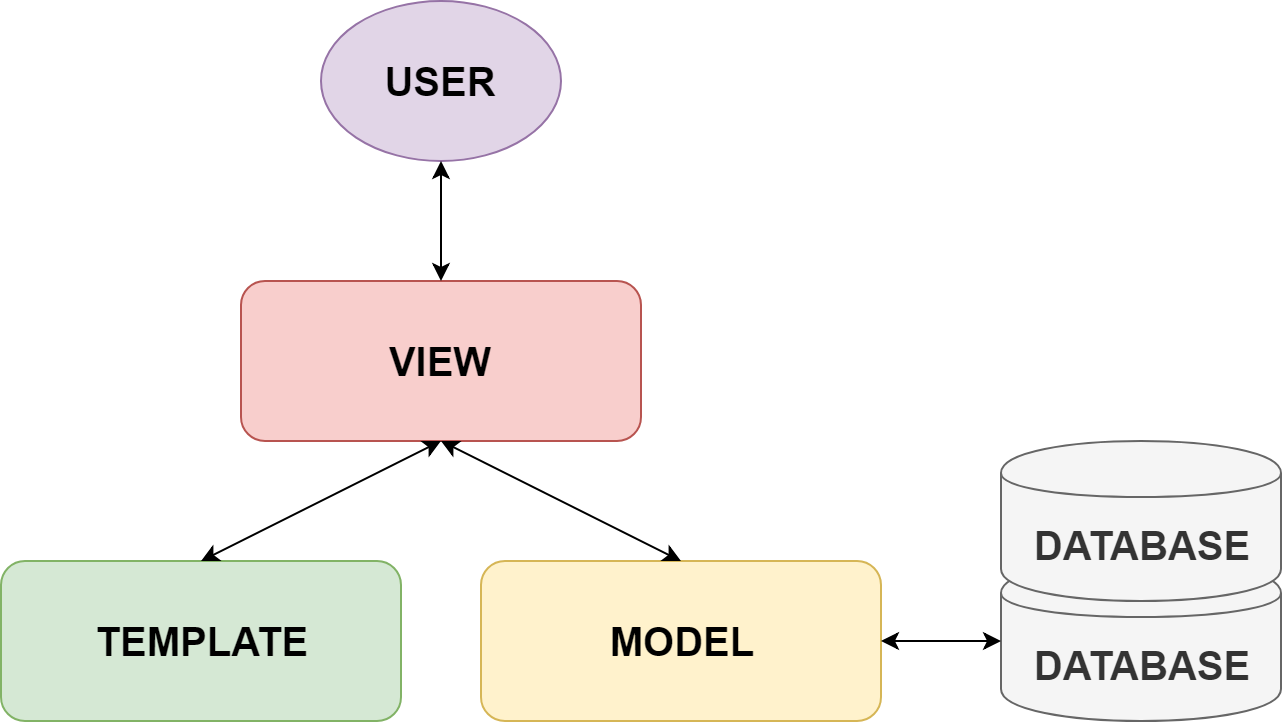
\includegraphics[width=120mm]{images/mtv.png}
		\caption{Mô hình MTV trong Django}
	\end{figure}
\end{center}
\par
Trong đó:
\begin{itemize}
	\item Model (M): Xử lý biểu diễn dữ liệu của bạn, nó được thể hiện như một giao diện cho dữ liệu được lưu trữ trong cơ sở dữ liệu và cũng cho phép bạn tương tác với dữ liệu của mình mà không phải cần kiến thức về các lệnh cơ sở dữ liệu.
	\item Template (T): Đại diện cho những gì bạn thấy trên trình duyệt cho ứng dụng web.
	\item View (V): Cung cấp logic để xử lý luồng dữ liệu trong chế độ xem hoặc cập nhật dữ liệu của Model, nó sử dụng logic được lập trình để tìm ra những gì được chuyển từ cơ sở dữ liệu thông qua Model và chuyển đến Template. Ngoài ra, nó có thể nhận thông tin từ người dùng thông qua Template và thực hiện logic đã cho bằng cách thay đổi chế độ xem hoặc cập nhật dữ liệu qua Model.
\end{itemize}
\subsubsection{Cấu trúc dự án và ứng dụng}
Một project của Django (ví dụ, \textbf{\texttt{lvtn}}) sẽ có cấu trúc và chức năng như sau:
\begin{lstlisting}
lvtn\
	lvtn\
		__init__.py
		settings.py
		urls.py
		wsgi.py
	manage.py
\end{lstlisting}
\par
Trong đó:
\begin{itemize}
	\item \texttt{manage.py}: Một CLI giúp tương tác với ứng dụng web.
	\item \texttt{lvtn\textbackslash\_\_init\_\_.py}: File rỗng, để chỉ cho Python biết thư mục này nên được xem là một gói.
	\item \texttt{lvtn\textbackslash settings.py}: Chứa các tùy chỉnh của project.
	\item \texttt{lvtn\textbackslash urls.py}: Các khai báo URL cho trang web.
	\item \texttt{lvtn\textbackslash wsgi.py}: Được sử dụng khi deploy project lên Internet.
\end{itemize}
\par
Server phát triển: Dùng để khởi chạy ứng dụng website trên máy tính local. Khi server đang chạy, truy cập vào địa chỉ \url{http://localhost:8000} trên trình duyệt để thấy ứng dụng đang được chạy.
\par
Tạo app mới: Mỗi ứng dụng được viết trong Django sẽ tuân thủ theo một quy ước nhất định. Django đi kèm với một tiện ích tự động tạo cấu trúc thư mục cơ bản của một ứng dụng, do đó người lập trình chỉ cần quan tâm đến việc phát triển code bên trong mà thôi.
\par
Một app (ví dụ, \textbf{\texttt{checkweb}}) trong project của Django được tạo ra có cấu trúc như sau:
\begin{lstlisting}
checkweb\
	migrations\
		__init__.py
	__init__.py
	admin.py
	apps.py
	models.py
	tests.py
	views.py
\end{lstlisting}
\par
Trong đó:
\begin{itemize}
	\item \texttt{migrations\textbackslash}: Thư mục chứa các file được sinh ra khi có thay đổi về cấu trúc cơ sở dữ liệu.
	\item \texttt{admin.py}: Dùng để thiết đặt các thuộc tính được hiển trị trong trang quản trị admin mà Django cung cấp sẵn.
	\item \texttt{apps.py}: Khai báo app được sử dụng trong project, đảm bảo rằng các app không bị trùng lặp trong 1 dự án.
	\item \texttt{models.py}: Django hỗ trợ các phương thức để xử lý cơ sở dữ liệu mà không cần sử dụng đến các câu lệnh truy vấn SQL trực tiếp.
	\item \texttt{tests.py}: Được người dùng sử dụng để triển khai các kịch bản thử nghiệm và rà soát lỗi trước khi phát hành ứng dụng.
	\item \texttt{views.py}: Đóng vai trò xử lý trung tâm của ứng dụng, quản lý việc hiển thị, kết nối đến cơ sở dữ liệu và thực thi các hàm do lập trình viên thêm vào ứng dụng.
\end{itemize}
\par
Sau khi tạo xong app, cần phải khai báo trong project bằng các thêm dòng sau vào file \texttt{lvtn\textbackslash settings.py}:
\begin{lstlisting}[language=Python]
INSTALLED_APPS = [
    "django.contrib.admin",
    "django.contrib.auth",
    "django.contrib.contenttypes",
    "django.contrib.sessions",
    "django.contrib.messages",
    "django.contrib.staticfiles",
    # add code below
    "checkweb.apps.CheckwebConfig",
]
\end{lstlisting}
\par
Class-based view: Đây là chức năng được Django hỗ trợ, giúp lập trình viên ít phải viết code hơn để hiện thị một giao diện lên trình duyệt web. Nó hỗ trợ tốt trong việc truyền tham số, lấy giá trị từ model và có thể dễ dàng tùy chỉnh theo ý muốn.
\par
Để sử dụng, cần phải thêm module vào file muốn dùng nó. Đoạn code sau có chức năng hiển thị file \textbf{\texttt{about.html}} ra đường dẫn \url{http://localhost:8000/about/}.
\begin{lstlisting}[language=Python]
from django.urls import path
from django.views.generic import TemplateView

urlpatterns = [
	path("about/", TemplateView.as_view(template_name="about.html")),
]
\end{lstlisting}
\par
Django template: Dựa trên file \textbf{\texttt{.html}} nhưng có chèn thêm các đoạn code riêng biệt để mỗi khi chạy chương trình, Django sẽ render ra giao diện lên trình duyệt tương ứng.
\begin{lstlisting}[language=HTML]

{{ section.title }}

<h1>{{ section.title }}</h1>

<h2>
 	<a href="{{ story.get_absolute_url }}">
		{{ story.headline|upper }}
	</a>
</h2>
<p>{{ story.tease|truncatewords:100 }}</p>


\end{lstlisting}
\section{Thư viện Python}
\subsection{Requests}
Requests là một thư viện HTTP thanh lịch và đơn giản viết bằng Python, được xây dựng dành cho con người\cite{requests}.
\par
Phiên bản sử dụng: 2.21.0
\par
Cách cài đặt:
\begin{lstlisting}[language=bash]
\>pip install requests
\end{lstlisting}
\par
Phương thức \textbf{\texttt{get}}: Dùng để lấy toàn bộ nội dung trang web dựa trên tham số url.
\begin{lstlisting}[language=Python]
import requests
page = requests.get(url)
\end{lstlisting}
\subsection{Lxml}
Lxml là thư viện được sử dụng để phân tách các thành phần trong mã nguồn nhằm hỗ trợ cho cú pháp \textbf{\texttt{xpath}} lấy nội dung từ website\cite{lxml}.
\par
Phiên bản sử dụng: 4.3.3
\par
Cách cài đặt:
\begin{lstlisting}[language=bash]
\>pip install lxml
\end{lstlisting}
Gói \texttt{lxml.html}: Dùng để phân tách chuỗi HTML.
\begin{lstlisting}[language=Python]
from lxml import html
content = html.fromstring(page.content)
value = content.xpath("//title/text()")
\end{lstlisting}
\subsubsection{Cú pháp phân tích sử dụng xpath}
XPath sử dụng các biểu thức đường dẫn để chọn các nút hoặc tập hợp nút trong tài liệu XML. Các biểu thức đường dẫn này trông rất giống với các biểu thức đường dẫn bạn sử dụng với các hệ thống tệp máy tính truyền thống. Trong dự án, chúng tôi dùng để phân tích cú pháp HTML\cite{xpath}.
\par
Cú pháp chọn nút
\begin{table}[!ht]
	\centering
	\begin{tabular}{|c|l|}
		\hline
		nodename & Chọn tất cả các nút có tên là "nodename"\\
		\hline
		/ & Chọn từ nút gốc\\
		\hline
		// & Chọn các nút từ nút hiện tại khớp với lựa chọn bất kể chúng ở đâu\\
		\hline
		. & Chọn nút hiện tại\\
		\hline
		.. & Chọn nút cha của nút hiện tại\\
		\hline
		@ & Chọn thuộc tính trong thẻ\\
		\hline
	\end{tabular}
	\caption{Cú pháp chọn nút trong xpath}
\end{table}
\section{Thư viện giao diện}
\subsection{Bootstrap}
Bootstrap là một thư viện HTML, CSS và JavaScript phổ biến trên thế giới để xây dựng nên các website có giao diện đáp ứng trên nhiều kích cỡ thiết bị khác nhau\cite{bootstrap}.
\par
Phiên bản sử dụng: 4.3.1
\par
Cách sử sử dụng Bootstrap vào website:
\begin{itemize}
 	\item CSS: Sao chép và dán dòng code bên dưới vào trong thẻ \texttt{<head>} trước tất cả các định dạng khác để tải CSS của Bootstrap.
 	\begin{lstlisting}[language=HTML]
<link rel="stylesheet" href="https://stackpath.bootstrapcdn.com/bootstrap/
4.3.1/css/bootstrap.min.css">
	\end{lstlisting}
	\item JS: Đặt trong thẻ \texttt{<script>} ở gần cuối trang web, trước khi đóng thẻ \texttt{</body>} để kích hoạt chúng. jQuery phải được đặt trước, đến Popper.js và sau cùng là phần JavaScript.
	\begin{lstlisting}[language=HTML]
<script src="https://code.jquery.com/jquery-3.3.1.slim.min.js"></script>
<script src="https://cdnjs.cloudflare.com/ajax/libs/popper.js/1.14.7/umd/
popper.min.js"></script>
<script src="https://stackpath.bootstrapcdn.com/bootstrap/4.3.1/js/
bootstrap.min.js"></script>
	\end{lstlisting}
\end{itemize}
\subsection{Font Awesome}
Font Awesome là thư viện miễn phí cung cấp các icon dạng vector và các logo xã hội lên website\cite{awesome}.
\par
Phiên bản sử dụng: 5.8.2
\par
Trước khi sử dụng được, cần phải chèn dòng code bên dưới vào thẻ \texttt{<head>} nằm ở đầu trang web.
\begin{lstlisting}[language=HTML]
<link rel="stylesheet" href="https://use.fontawesome.com/releases/v5.8.2/css/
all.css">
\end{lstlisting}
\par
Để chèn icon vào trang web, sử dụng dòng code tương tự cú pháp bên dưới:
\begin{lstlisting}[language=HTML]
<i class="fas fa-heart"></i>
\end{lstlisting}
\section{reCAPTCHA}
reCAPTCHA là một dịch vụ miễn phí bảo vệ website tránh khỏi spam và lạm dụng\cite{captcha}.
\par
Phiên bản sử dụng: reCAPTCHA v2 Invisible
\par
Cách đơn giản để sử dụng reCAPTCHA vào trang web bằng cách nhúng mã JavaScript và thẻ \texttt{g-recaptcha}. Thẻ \texttt{g-recaptcha} là 1 thẻ \textbf{\texttt{button}} với tên class là \texttt{"g-recaptcha"}, có thuộc tính \texttt{data-sitekey} chứa Site key được cấp khi đăng ký sử dụng reCAPTCHA.
\begin{lstlisting}[language=HTML]
<html>
  	<head>
    	<title>reCAPTCHA demo: Simple page</title>
     	<script src="https://www.google.com/recaptcha/api.js" async defer></script>
     	<script>
       	function onSubmit(token) {
         	document.getElementById("demo-form").submit();
       	}
     	</script>
  	</head>
  	<body>
    	<form id="demo-form" action="?" method="POST">
      	<button class="g-recaptcha" data-sitekey="your_site_key" data-callback="onSubmit">Submit</button>
      	<br/>
    	</form>
  	</body>
</html>
\end{lstlisting}
\par
Sau khi submit form sử dụng reCAPTCHA, cần phải gửi giá trị có tên là \texttt{g-recaptcha-\\response} bằng phương thức POST về máy chủ của Google để xác minh người dùng đã xác thực bằng reCAPTCHA tại địa chỉ \url{https://www.google.com/recaptcha/api/siteverify}.
\begin{itemize}
	\item secret (bắt buộc): Khóa Secret key được cấp đồng thời với Site key khi đăng ký sử dụng.
	\item response (bắt buộc): Kết quả trả về của thuộc tính có tên là \texttt{g-recaptcha-response}.
	\item remoteip: Địa chỉ IP của người dùng cuối.
\end{itemize}
\par
Tiếp theo, Google sẽ trả về kết quả kiểm tra có thỏa reCAPTCHA dưới dạng JSON bằng các giá trị sau:
\begin{lstlisting}[language=Python]
{
	"success": true|false,
	"challenge_ts": timestamp, # timestamp of the challenge load
	"hostname": string, # the hostname of the site where the reCAPTCHA was solved
	"error-codes": [...] # optional
}
\end{lstlisting}
\par
Dựa vào kết quả này, chúng tôi có thể biết được người dùng đã có giải được captcha hay chưa, sau đó tiến hành các yêu cầu từ người dùng.	
\section{Heroku platform}
Heroku là một nền tảng đám mây cho phép xây dựng, phân phối, giám sát và mở rộng ứng dụng\cite{heroku}.
\par
Đầu tiên và quan trọng nhất, các ứng dụng Heroku yêu cầu một file \texttt{Procfile} để cài đặt nền tảng sử dụng, được đặt tại thư mục gốc.
\par
\texttt{Procfile}
\begin{lstlisting}[language=sh]
web: gunicorn myproject.wsgi
\end{lstlisting}
\par
File \texttt{Procfile} này yêu cầu \texttt{Gunicorn}, 1 máy chủ web được khuyến nghị dùng cho ứng dụng Django. Để cài đặt, sử dụng lệnh:
\begin{lstlisting}[language=bash]
\>pip install gunicorn
\end{lstlisting}
\par
Thay đổi trong file \texttt{settings.py} của ứng dụng Django. Khi sử dụng Heroku, các thông tin nhạy cảm sẽ được lưu trữ trong môi trường được gọi là config vars. Nó bao gồm các thông tin để kết nối đến cơ sở dữ liệu, trong khi bình thường sẽ được ghi trong file \texttt{settings.py} của Django.
\par
Gói \texttt{django-heroku} sẽ tự động cấu hình ứng dụng Django để nó hoạt động trên Heroku. Nó tương thích với các ứng dụng Django 2.0. Để cài đặt, sử dụng lệnh:
\begin{lstlisting}[language=bash]
\>pip install django-heroku
\end{lstlisting}
\par
Sau khi cài đặt, cần phải \texttt{import} câu lệnh sau vào đầu file \texttt{settings.py}:
\begin{lstlisting}[language=Python]
import django_heroku
\end{lstlisting}
\par
Sau đó thêm phần sau vào cuối file \texttt{settings.py}:
\begin{lstlisting}[language=Python]
# activate django-heroku.
django_heroku.settings(locals())
\end{lstlisting}